\chapter{Konstruktion des Vergleichssegments}\label{cha:Konstruktion des Vergleichssegments}

\section{Modellaufbau}

Aufgrund der symetrischen Auslegung des Tragwerks wir im CAD Modell zunächst nur eine Halbspannweite Modelliert.

Ausgehend von der Wurzelrippe wird hier die Variante mit Rohrholm aus dem Werkstoff 3.1354 dargestellt.

\begin{figure}[H]
\centering
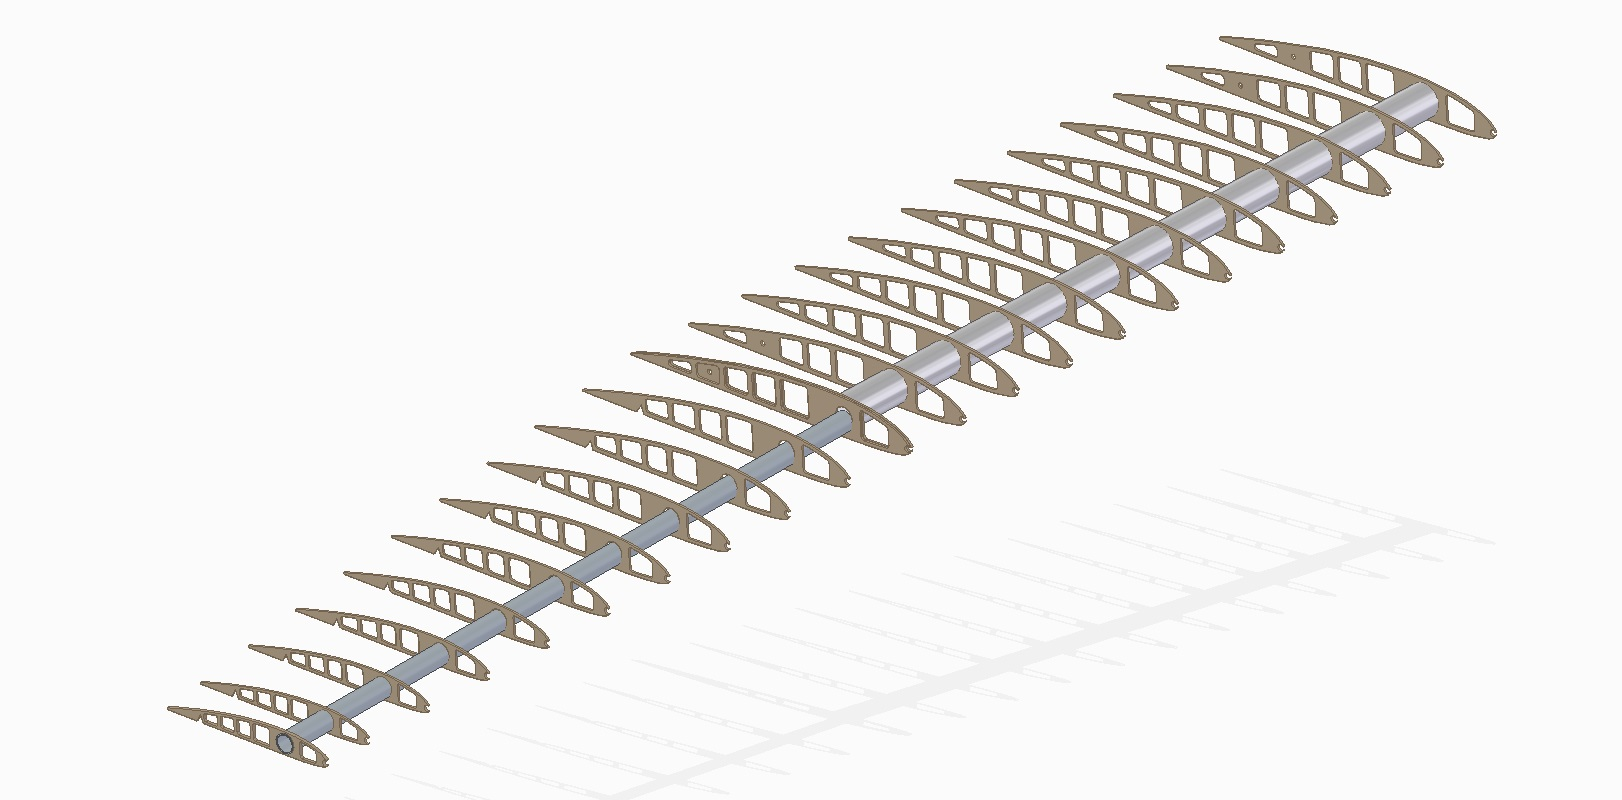
\includegraphics[width=0.9\textwidth]{bilder/Fotos/Halbspannweite.png}
\caption{Screenshot aus der Baugruppen CAD Darstellung} 
\label{fig:Screenshot aus der Baugruppen CAD Darstellung}
\end{figure}

Es handelt sich hierbei um eine Rohrholm-Rippen-Bauweise, wobei die Rippen auf das Aluminium Rundrohr aufgefädelt und verklebt werden.